\documentclass[12pt]{article}

\usepackage[utf8]{inputenc}
\usepackage[a4paper, margin=1in]{geometry}
\usepackage{booktabs}
\usepackage{physics}
\usepackage{amsmath}
\usepackage{amsfonts}
\usepackage{graphicx}
\usepackage{siunitx}
\usepackage{multirow}

\graphicspath{{./figures}}

\title{Physical Climatology (AES 630) Project 2}
\author{Mitchell Dodson}
\date{October 16, 2023}

\newcommand*{\problem}[2]{
    \begin{table}[ht]
    \centering
        \begin{tabular}{ | p{.1\linewidth} p{.9\linewidth} | }
            \hline
            \vspace{.3em}\textbf{\large#1:} & \vspace{.3em}\footnotesize{#2}\hspace{.2em}\vspace{.5em} \\ \hline
        \end{tabular}
    \end{table}
}


\newcommand\T{\rule{0pt}{2.6ex}}       % Top strut
\newcommand\B{\rule[-1.2ex]{0pt}{0pt}} % Bottom strut

\begin{document}

\vspace{-2em}

\maketitle

\vspace{-2em}

\problem{1,2}{
    \footnotesize
    Include the value of HF in your EBM3o model and recalculate the temperatures of
    the three layers using the radiative transfer coefficients applied in the first homework
    assignment(i.e. far right column of Table 2). This basic version of your model, which includes
    HF, will be known as EBM3HF. Use the radiation coefficients of Kiehl and Trenberth 2 and solve
    for the temperatures of the three layers (include HF.)}

\begin{figure}[h!]\label{q1q2}
    \centering
    \begin{tabular}{ r | c | c c c}
        Model & Metric & Layer 1 & Layer 2 & Surface \T\B\\
        %\hline
        %\multicolumn{4}{c}{EBM3} \\
        \hline
        \multirow{2}*{EBM3$_0$} &
        Absorption ($\si{W.m^{-2}}$) & 8.714 & 59.969 & 170.158 \T\\
        & Temperature ($\si{K}$) & 233.716 & 269.503 & 308.461 \B\\
        %\hline
        %\multicolumn{4}{c}{EBM3 with Heat Flux} \\
        \hline
        \multirow{2}*{EBM3$_{HF}$} &
        Absorption ($\si{W.m^{-2}}$) & 8.713 & 158.859 & 71.268 \T\\
        & Temperature ($\si{K}$) & 233.716 & 271.120 & 287.295 \B\\
        \hline
        %\multicolumn{4}{c}{Kiehl and Trenberth 2} \\
        %\hline
        \multirow{2}*{K$\&$H 2} &
        Absorption ($\si{W.m^{-2}}$) & 10.547 & 174.976 & 48.809 \T\\
        & Temperature ($\si{K}$) & 243.985 & 286.226 & 286.587 \B\\
    \end{tabular}
    \caption{Layerwise equilibrium temperature and absorption of shortwave solar and heat flux energy for each of the coefficient sets of the 3-layer energy-based model. The absorption results for EBM3$_{HF}$ and Kiehl$\&$Trenberth 2 (K$\&$H 2) include heat flux from the surface to layer 2 such that HF$:=.29Q$ for average solar irradiance $Q=341\,\si{W.m^{-2}}$.}
\end{figure}


\problem{3}{
    \footnotesize
    For this problem, use your EBM3HF radiative transfer coefficients from Problem 1
    above with the HF component included (i.e. EBM3HF). The task is to mimic a changing
    greenhouse effect within a single atmospheric layer in this model. Start with EBM3HF but with a2
    = 0.720, then increase a2 by steps of 0.002 from 0.710 to 0.770 while at the same time reducing
    the transmissivity t2 from 0.075 to 0.015 while leaving r2 the same (i.e. a2 + t2 = 0.785). Solve for
    the temperature of the three layers as a2 and t2 change by small increments. Plot the results
    with the absorption a 2 on the x-axis and the temperatures on the y-axis.
    What is the effect of making the troposphere (level 2) more absorptive to thermal radiation on all levels
    (i.e.  analogous to increasing the greenhouse effect)?
    What is the average linear rate of surface temperature change ($\Delta$T3 ) relative to a change in a2
    ($\Delta$a2 ) over this range (i.e., $\Delta$T3 /$\Delta$a2 )?
    What are the rates of change for T1 and T2 , (i.e. $\Delta$T1 /$\Delta$a2 , and $\Delta$T2 /$\Delta$a2 )?
    What happens to the tropospheric lapse rate (T3 -T2 ) as a2 increases? What else could change
    (feedback) that would keep the tropospheric lapse rate near that of the base case?}

\clearpage

\begin{figure}[h!]
    \centering
    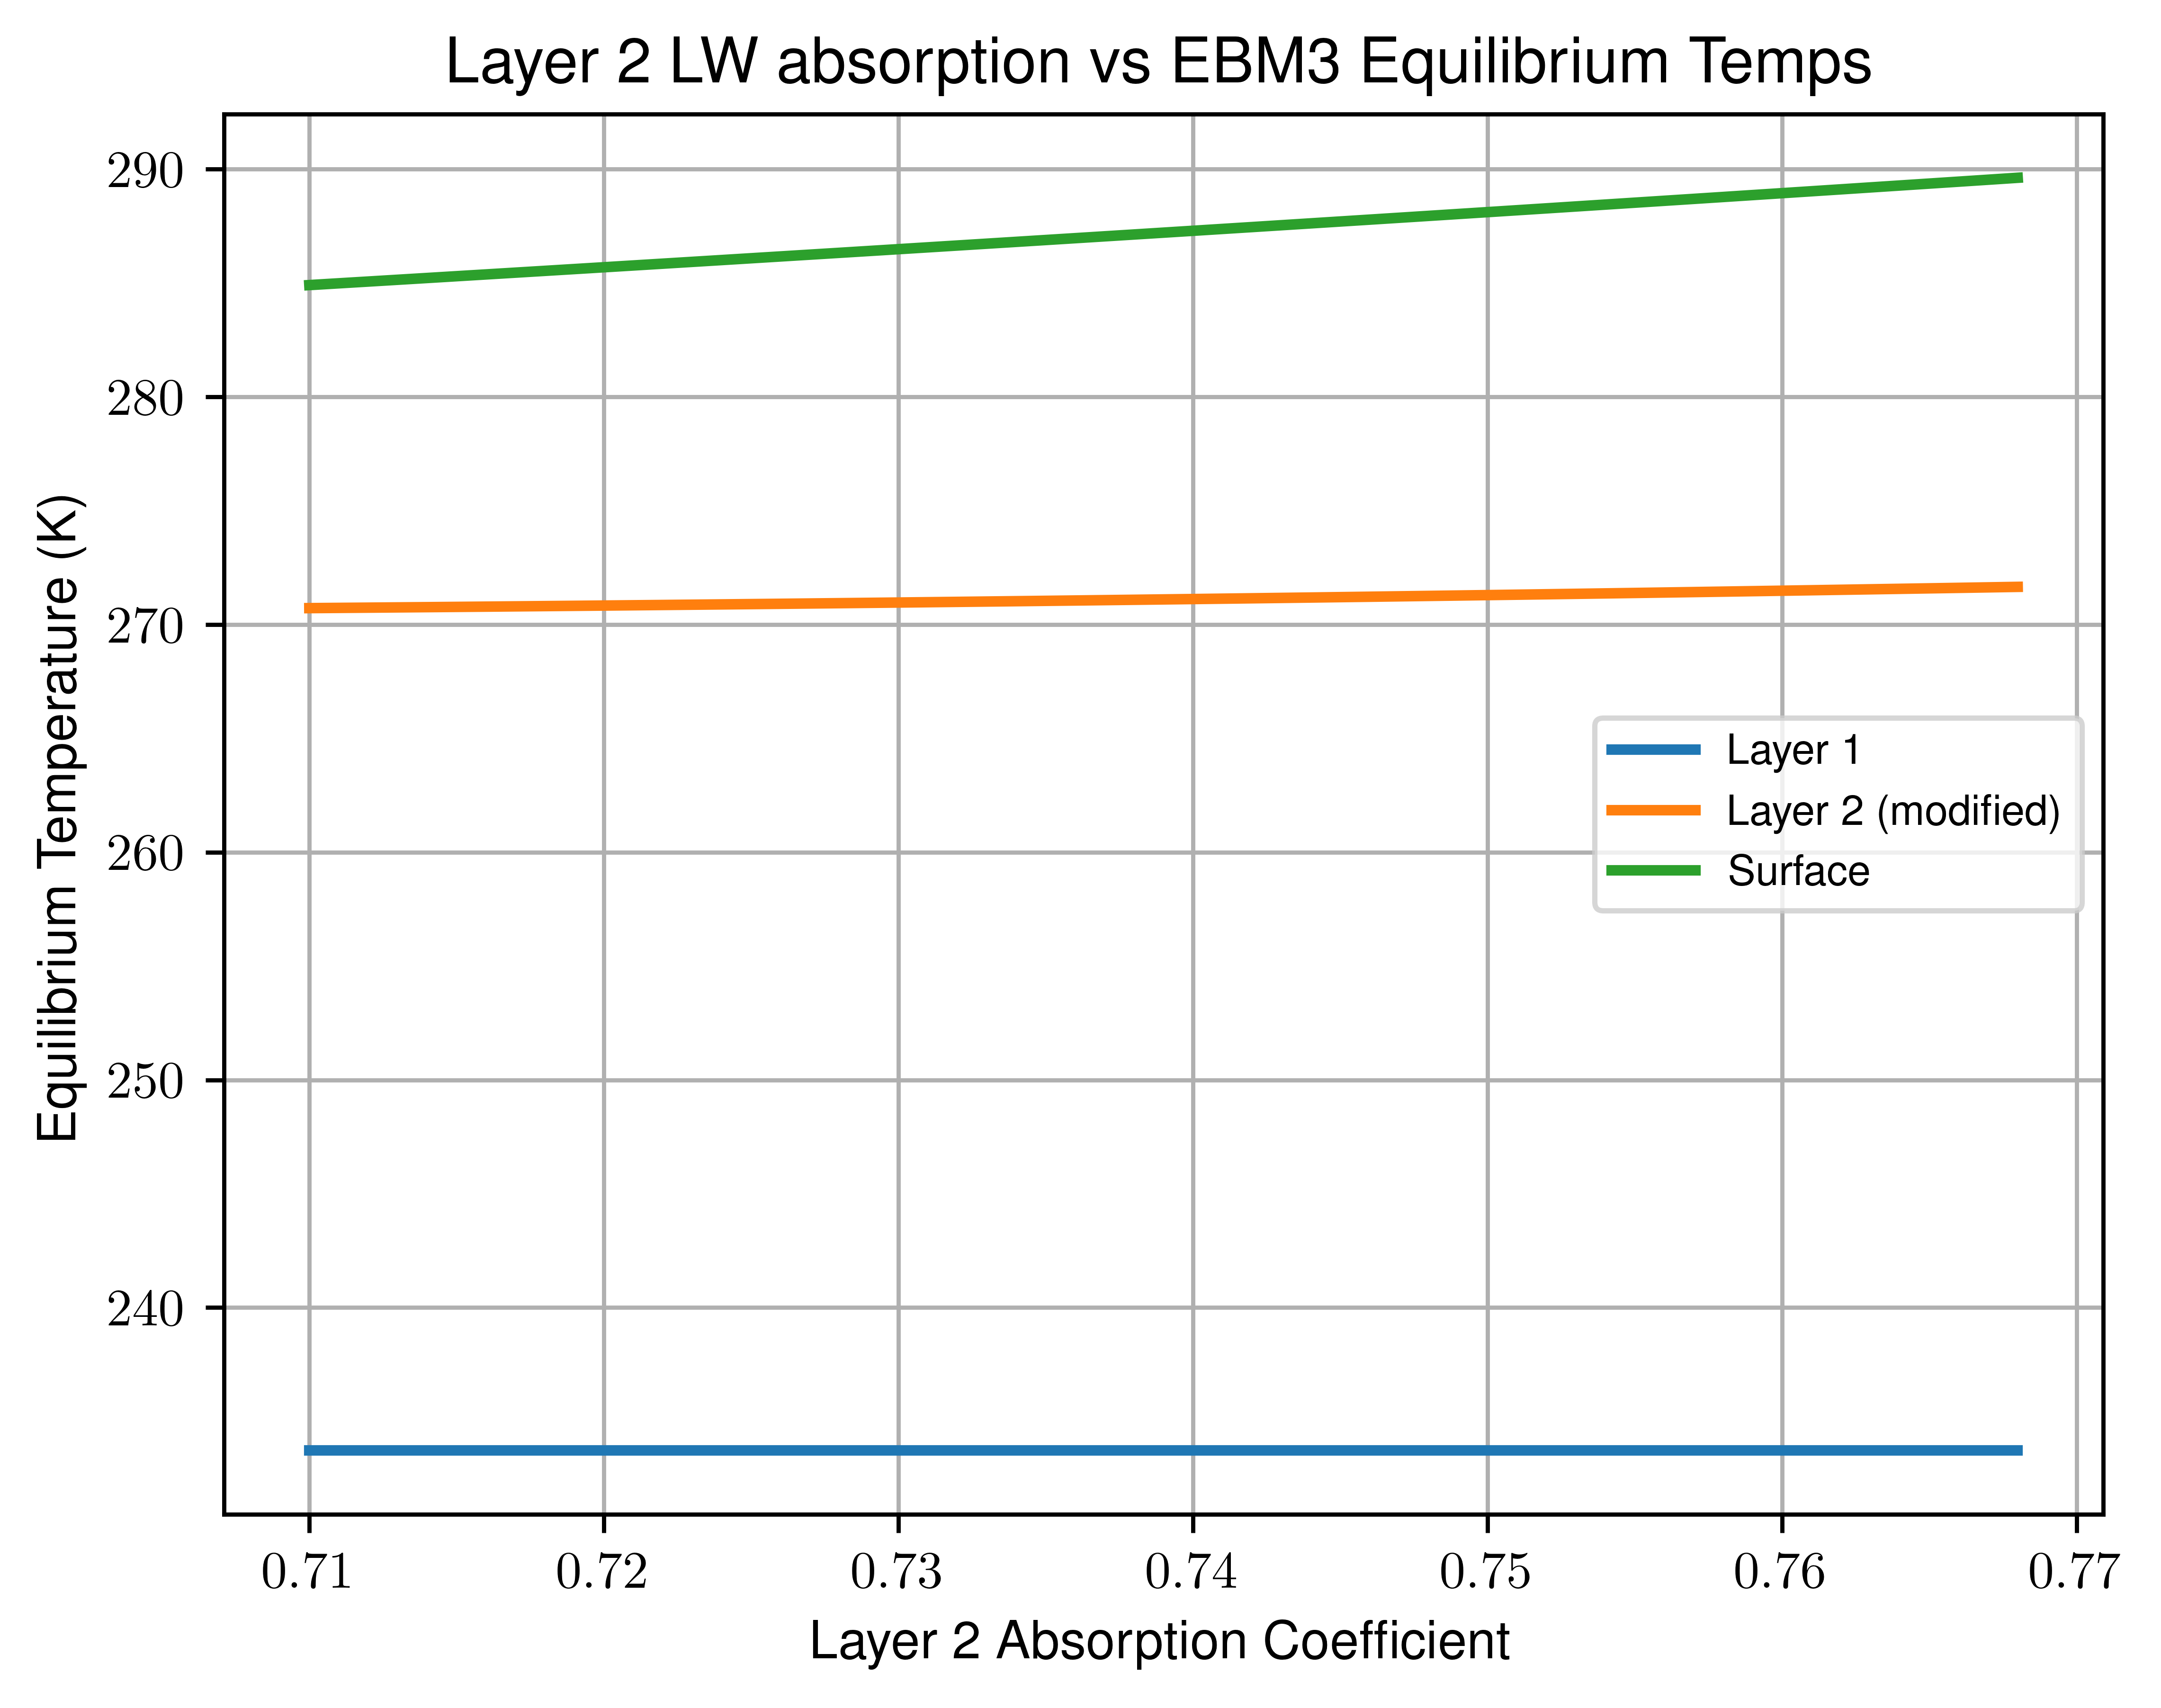
\includegraphics[width=.70\linewidth]{ebm3hf_dTda_l2.png}
    \caption{Change in equilibrium temperatures of each layer in the EBM3$_0$ model as the layer 2 absorption increases, and transmissivity decreases. The average rate of change in surface temperature for layers 1-3 ($\frac{dT}{d\alpha_2}$) are $0.000\,\si{K}$, $16.098\,\si{K}$, and $81.265\,\si{K}$ per unit increment in absorptivity, respectively. These were calculated by averaging the elementwise forward-difference and dividing by the total change in absorption.}
    \label{dtdal2}
\end{figure}

Figure \ref{dtdal2} displays my results when varying the layer 2 thermal absorptivity and transmissivity by increments of .002.  Layer 2 increased in temperature from $270.37\,\si{K}$ to $271.76\,\si{K}$, and layer 3 (surface) increased from $286.67\,\si{K}$ to $287.835\,\si{K}$. The temperature of layer 1 was unaffected by the modified layer 2 absorption, which was surprising to me since the radiative model for the top-most layer is functionally dependent on layer 2's absorptivity and transmissivity. Nonetheless, I confirmed that the coefficient matrix components corresponding to layer 1 change along with the layer 2 absorption/transmission.

Since only the thermal absorptivity and transmissivity were modified, and shortwave properties remain the same in all the layers, the total emission temperature of the planet must stay constant as absorptivity in layer 2 increases. The temperature at layer 2 is a larger component of the planetary emission temperature as it becomes more opaque because it emits more efficiently, and because emissions from the surface are more strongly attenuated and re-emitted by layer 2. In effect, this increases the total energy ``capacity'' of the toposphere, which is the phenomenon described by the greenhouse effect. Assuming layer altitudes remain consistent, the lapse rate in the troposphere at equilibrium increases accordingly.

Changes in the planetary radiative properties that could help re-establish the original lapse rate given stronger layer 2 absorption include an increase in shortwave reflectivity at layer 1, which causes less total insolation to be introduced to the lower atomsphere (as is the case when sulfate aerosols are introduced to the upper atmosphere after volcanic eruptions). Modifying layer 1 of my EBM3$_0HF$ model such that shortwave reflectivity $\rho = .238$ rather than $\rho = 0.038$, and transmissivity $\tau = .742$ rather than $\tau=.942$ caused the temperature difference between the surface and layer 2 to remain consistent between the cases at about $13\,\si{K}$. An increase in the layer 2 or surface shortwave reflectivity has a similar effect. In reality, the dominant mechanisms that establishes a consistent tropospheric lapse rate are sensible and latent heat fluxes, which generally move heat upward in exchange for downward mass flux in order to approach hydrostatic balance.

\problem{4}{
    Begin with EBM3HF of Problem 1 and change the value of a1 to mimic an increase in
    greenhouse gases in the stratosphere. In this case, start with a 1 at 0.070 and increase by 0.002
    increments to 0.120. Reduce t1 by the same amount, leaving r1 unchanged at 0.005 (so a1 + t1 = 0.995).
    Plot the values with a1 on x-axis and temperatures on y-axis.
    What is the average linear rate of surface temperature change ($\Delta$T3 ) relative to a change in a1
    ($\Delta$a1 ) over this range ($\Delta$T3 /$\Delta$a1 )?
    What is the rate of change for T1 and T2 , (i.e. ($\Delta$T1 /$\Delta$a1, and $\Delta$T2 /$\Delta$a1 )?}

\begin{figure}[h!]\label{dtdal1}
    \centering
    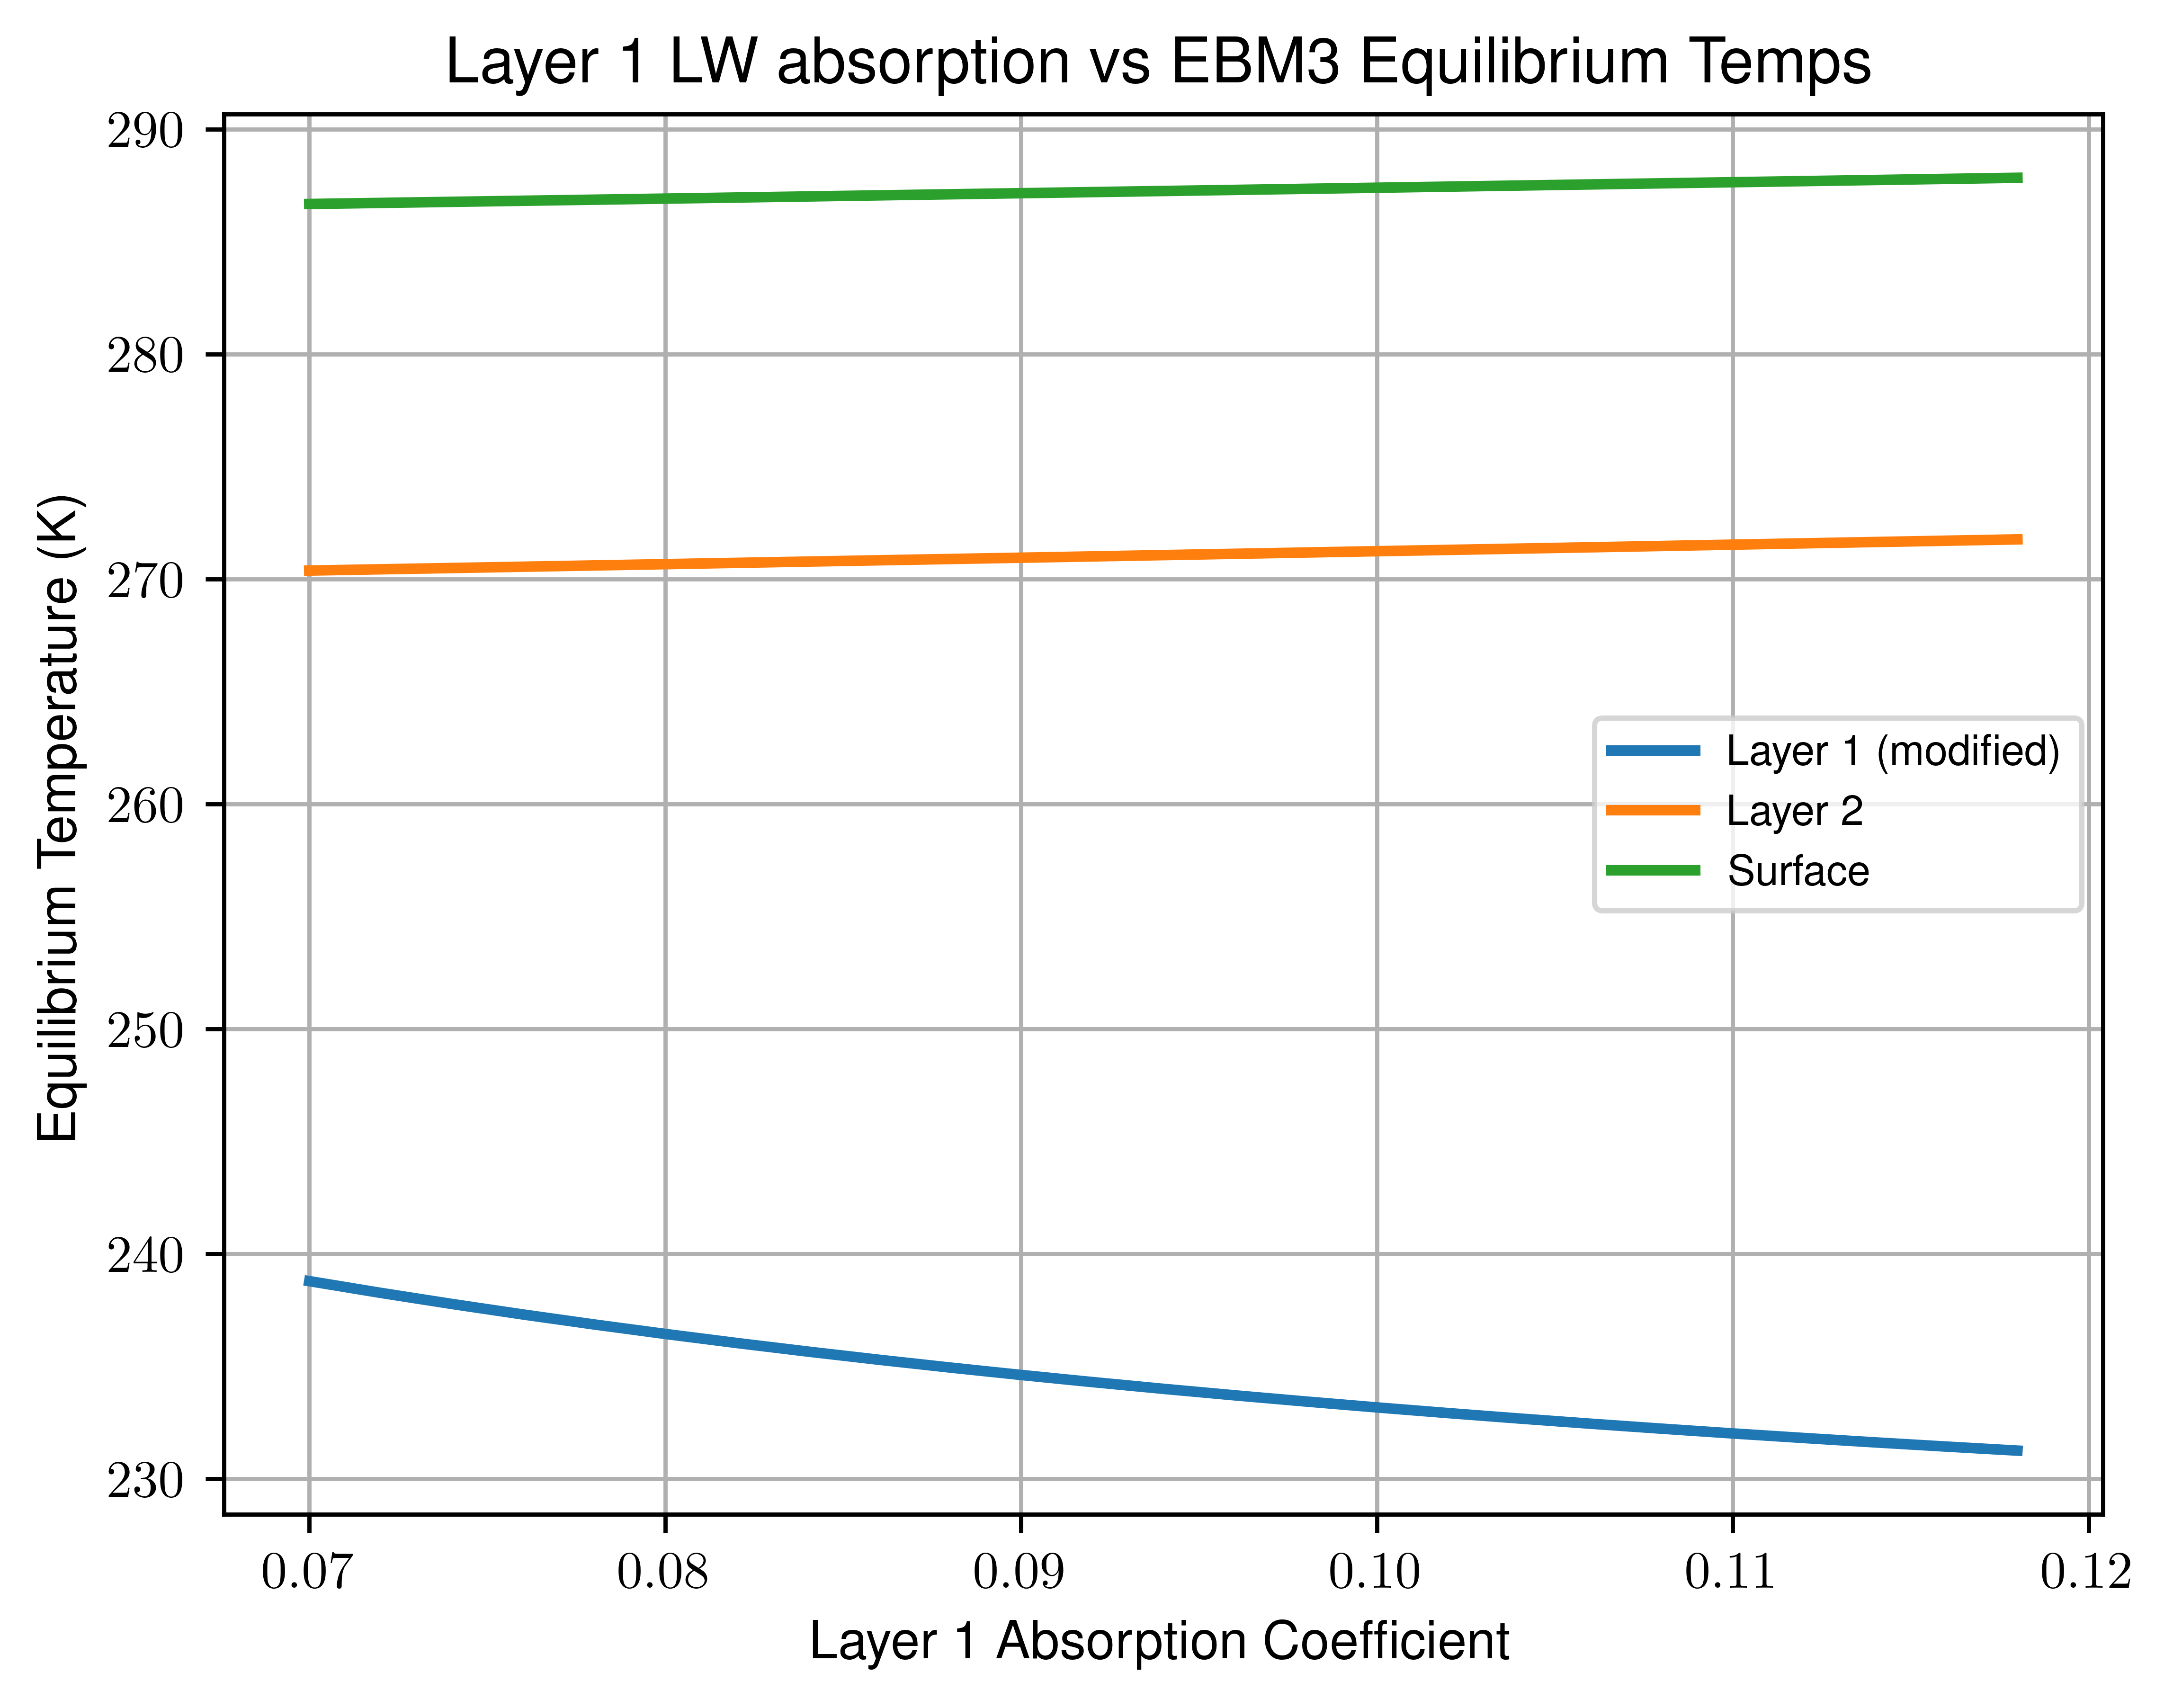
\includegraphics[width=.70\linewidth]{ebm3hf_dTda_l1.png}
    \caption{Equilibrium temperatures of each layer given increasing layer 1 longwave absorption, and decreasing transmission. The average linear rates of change (calculated with forward-differencing) are $-156.941\,\si{K}$, $28.881\,\si{K}$, and $24.270\,\si{K}$, respectively, however the layer 1 curve (and magnitude) makes it clear that the relationship is not linear. The rapid decrease in layer 1 temperature with additional thermal absorption is counterintuitive. Since longwave emissions incident on layer 1 only come from below, the additional absorption must cause the total amount of energy retained in the atmosphere to increase. This is because additional top-layer absorption can only decrease the amount of longwave radiation escaping to space from below. Shortwave interactions are unchanged, so the equilibrium emission temperature of Earth must be the same. Thus, as above, since the modified layer 1 contributes more to the emission temperature with greater absorption, the layer's equilibrium temperature should decrease substantially to offset the additional energy from below.}
\end{figure}


\end{document}
